\section{Experiments}
\label{sec:experiments}

We apply the developed methods to a vareity of datasets chosen to span a range of edge counts $E$ and feature-space dimension $D$. 
However, we first require metrics to assess model performance. This can be split into two separate 
components: the microcanonical SBM fit (concerned with the $b$-samples) and 
the fit of the feature-to-block generator (concerned with the $\theta$-samples). 

Starting with the SBM, recall that the quantity $S(b)$ in~(\ref{eqn:dl-form}) 
can be interpreted as an ideal ``description length'' of the partition 
imposed by $b$. We define the average
description length per entity (nodes and edges) $\bar{S}_e$ to gauge the SBM fit:
%
\begin{equation}
	\bar{S}_e \coloneqq \frac{1}{(N+E) |\Tcal_b|} \sum_{t\in \Tcal_b} S \left( b^{(t)} \right).
	\label{eqn:mean-dl}
\end{equation}

Next, to assess the performance of the feature-to-block predictor, 
we partition the vertex set $[N]$ into training and test sets. On each experiment run,
a constant fraction $f$ of the available vertices go to form 
the training set $\Gcal_0$ and the remainder are held out to form the
test set $\Gcal_1$. These sets are chosen randomly.
The $b$-chain is run using the whole network but we only use vertices $v \in \Gcal_0$ to train the $\theta$-chain. Because $|\Gcal_0| \neq |\Gcal_1|$ in general, we cannot use the un-normalised log-target $U$ from~(\ref{eqn:U-form}) for benchmarking,
as the total cross-entropy loss scales with the size of each data set but 
the prior term stays constant. We therefore use the average cross-entropy loss 
over each set,
%
\begin{equation}
	\bar{\Lcal}_\star \coloneqq \frac{1}{|\Tcal_\theta|} \sum_{t \in \Tcal_\theta} \Lcal_\star^{(t)},
	\quad \textrm{where} \quad
	\Lcal_\star^{(t)} \coloneqq \frac{1}{|\Gcal_\star|} \sum_{i \in \Gcal_\star}\sum_{j \in [B]} \hat{y}_{ij} \log \frac{1}{\phi_j \left(x_i; \theta^{(t)} \right)},
	\label{eqn:cross-entropy-loss}
\end{equation}
%
where $\star \in \{0, 1\}$ indicates whether the training or test
set is being considered.

Nevertheless, the cross-entropy loss over the whole training set may be too coarse a measure of model fit. It is often the case that we have good feature-based explanations for some but not all of the detected blocks. We wish to define a new measure of fit specific to each detected block. This requires defining the set of all vertices associated with block $j$ as,
$
	\Bcal_\star(j) \coloneqq \{i \in \Gcal_\star : \hat{b}_i = j\}
$
where
$ 
	\quad \hat{b}_i \coloneqq \argmax_j \hat{y}_{ij}.
$
Recall that $\hat{y}_{ij}$ is our estimate for the block membership posterior~(\ref{eqn:y-hat}) using only information from the adjacency matrix $A$. Again, $\star \in \{0, 1\}$ toggles between training and test sets. Now $\Bcal_\star(j)$ is the set of vertices that have maximum a posteriori probability of belonging to block $j$. We choose to resolve ties consistently by picking the lower index. We now define the accuracy for block $j$ as,
%
\begin{equation}
	\eta_\star(j) \coloneqq \frac{1}{|\Bcal_\star (j)| \cdot 
	|\Tcal_\theta| } 
	\sum_{i \in \Bcal_\star (j)}  \sum_{t \in \Tcal_\theta}
	\one \left\{\hat{b}_i = \argmax_j \phi_j \left( x_i; \theta^{(t)} \right) \right\}.
	\label{eqn:accuracy}
\end{equation}
%
This is effectively testing whether the feature-to-block and the graph-to=block predictions agree in their largest component. We call this metric, $\eta_\star(j)$, the {\em block-accuracy} for block $j$. It is clearly bounded $0 \leq \eta_\star(j) \leq 1$, with an accuracy of 1 meaning perfect agreement for the vertices in detected block $j$.

For each of the experiments, we plot the collected $\theta$-samples for the features that survive the dimensionality reduction procedure. We also plot the per-block accuracy for the original-dimension classifiers. We discuss the results specific to each dataset in turn.

Table~\ref{tab:results} summarises the results for each experiment. 
We see that the dimensionality reduction procedure 
brings the training and test losses closer together. This implies that 
the features we keep are indeed correlated with the underlying graphical 
partition and that the approach generalises correctly. The test loss variance is higher than the training loss variance as the test set is smaller and so more susceptible to variability in its construction.
%
The average description length per entity,
$\bar{S}_e$, of the graph, 
has very small variance, suggesting that
the detected communities can be found reliably (to within an arbitrary 
relabelling of blocks).

\paragraph{\textbf{Political books.}}

We choose to partition the network into $B=3$ communities as we only have this many distinct values for political affiliation.
From Figure~\ref{fig:polbooks-null} we see that all 3 blocks have a distinct political affiliation as their largest positive component.  
Furthermore, the training and test losses from Table~\ref{tab:results}  
are very similar and both are low in magnitude. This is strong evidence 
that political affiliation is a very appropriate explanatory 
variable for the overall network structure.
%
However, from Figure~\ref{fig:polbooks-accuracy} we see that block 1 has low accuracy. 
This suggests that detected block 1 is not solely composed of ``neutral" books but also 
contains some ``liberal" and ``conservative" authors. Examining 
Figure~\ref{fig:polbooks-graph}, we see the majority of paths between blocks 2 and 3 go through block 1.
Block 1 is in effect a bridge between the ``conservative'' and ``liberal'' blocks so it is unsurprising that some of these leak into block 1.

\paragraph{\textbf{Primary school.}}

We choose the number of communities $B=10$, in line with the total number of 
school classes. Only the pupils' class memberships (1A-5B) survive
the dimensionality-reduction process (Figure~\ref{fig:school-null});
gender and teacher/student status have been discarded,
meaning these are poor predictors of overall macro-structure.
%
The vast majority of blocks are composed of a single class. 
However, some blocks have two comparably strong classes as their predictors (e.g. blocks 2 and 5). 
Conversely, some classes are found to extend over two 
detected blocks (class 2B spans blocks 8 and 9) but we do 
not have a feature which explains the division.
%
Figure~\ref{fig:school-accuracy} shows excellent accuracy for the majority of blocks. In fact the only blocks with low accuracy are those that have a school-class span two blocks such that we cannot reliably distinguish between the two. This is more pronounced when we apply hard classification rather than the soft cross-entropy loss. Perhaps there are unobserved features which explain this divide.

\paragraph{\textbf{Facebook egonet.}}

The retained features 
(Figure~\ref{fig:fb-null}) are those that best explain the high-level 
community structure. The majority of these are education related. 
Nevertheless, for $D'=10$ we only have good explanations for some of the detected blocks; several blocks in 
Figure~\ref{fig:fb-null} do not have high-magnitude components. This is further emphasised by the disparate accuracies in Figure~\ref{fig:fb-accuracy}.
%
For a high-dimensional feature-space, it is likely that a particular
feature may uniquely identify a small set of vertices; if these are all in the same block, then the classifier may overfit despite the penalty imposed by the prior. Indeed, we see in
Figure~\ref{fig:fb-null} that the feature birthday-5 has a very high weight as it relates to block 1 – but it is unlikely that birthdays determine graphical structure.
\begin{table}[!ht]
	\centering
	\caption{Results averaged over $n=10$ iterations (mean $\pm$ std. dev.).}
	\label{tab:results}
	\resizebox{\textwidth}{!}{%
		\begin{tabular}{c|ccc|c|cc|ccc}
			Dataset  & $B$ & $D$ & $D'$ & $\bar{S}_e$ & $\bar{\mathcal{L}}_0$ & $\bar{\mathcal{L}}_1$ & $c^*$ & $\bar{\mathcal{L}}_0'$ & $\bar{\mathcal{L}}_1'$  \\ \hline
			Polbooks & 3 & 3 & -- & $2.250 \pm 0.000$ & $0.563 \pm 0.042$ & $0.595 \pm 0.089$ & -- & -- & -- \\
			School & 10 & 13 & 10 & $1.894 \pm 0.004$ & $0.787 \pm 0.127$ & $0.885 \pm 0.129$ & $1.198 \pm 0.249$ & $0.793 \pm 0.132$ & $0.853 \pm 0.132$ \\
			FB egonet & 10  & 480 & 10 & $1.626 \pm 0.003$ & $1.326 \pm 0.043$ & $1.538 \pm 0.069$ & $0.94 \pm 0.019$ & $1.580 \pm 0.150$ & $1.605 \pm 0.106$
		\end{tabular}
	}
\end{table}

\begin{figure}[!ht]
	\centering
	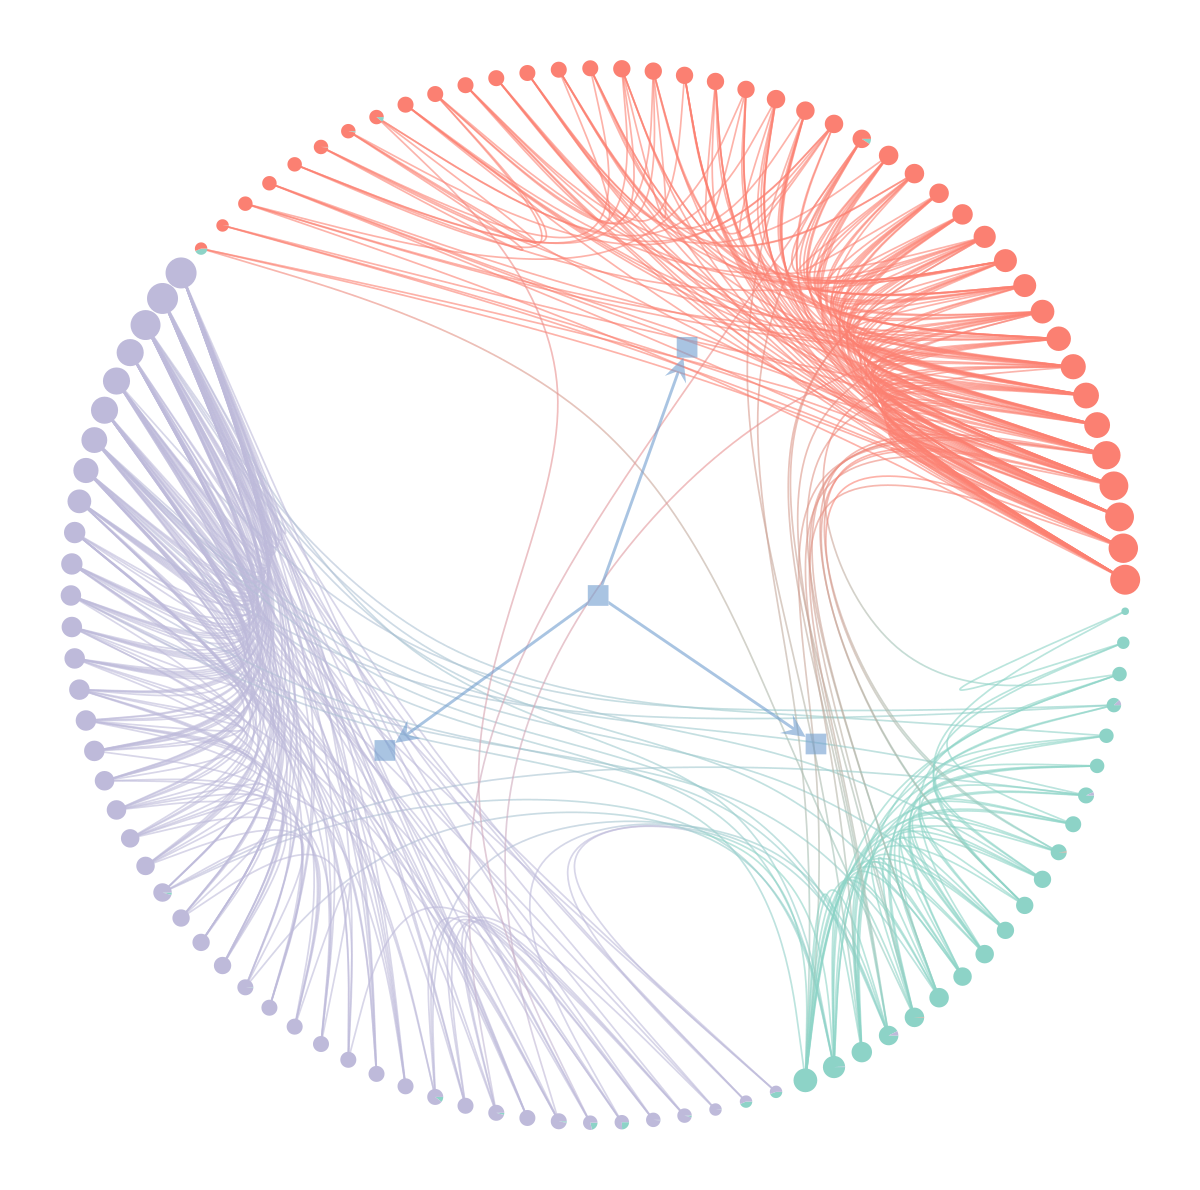
\includegraphics[width=0.28\linewidth]{img/polbooks-graph.png}
	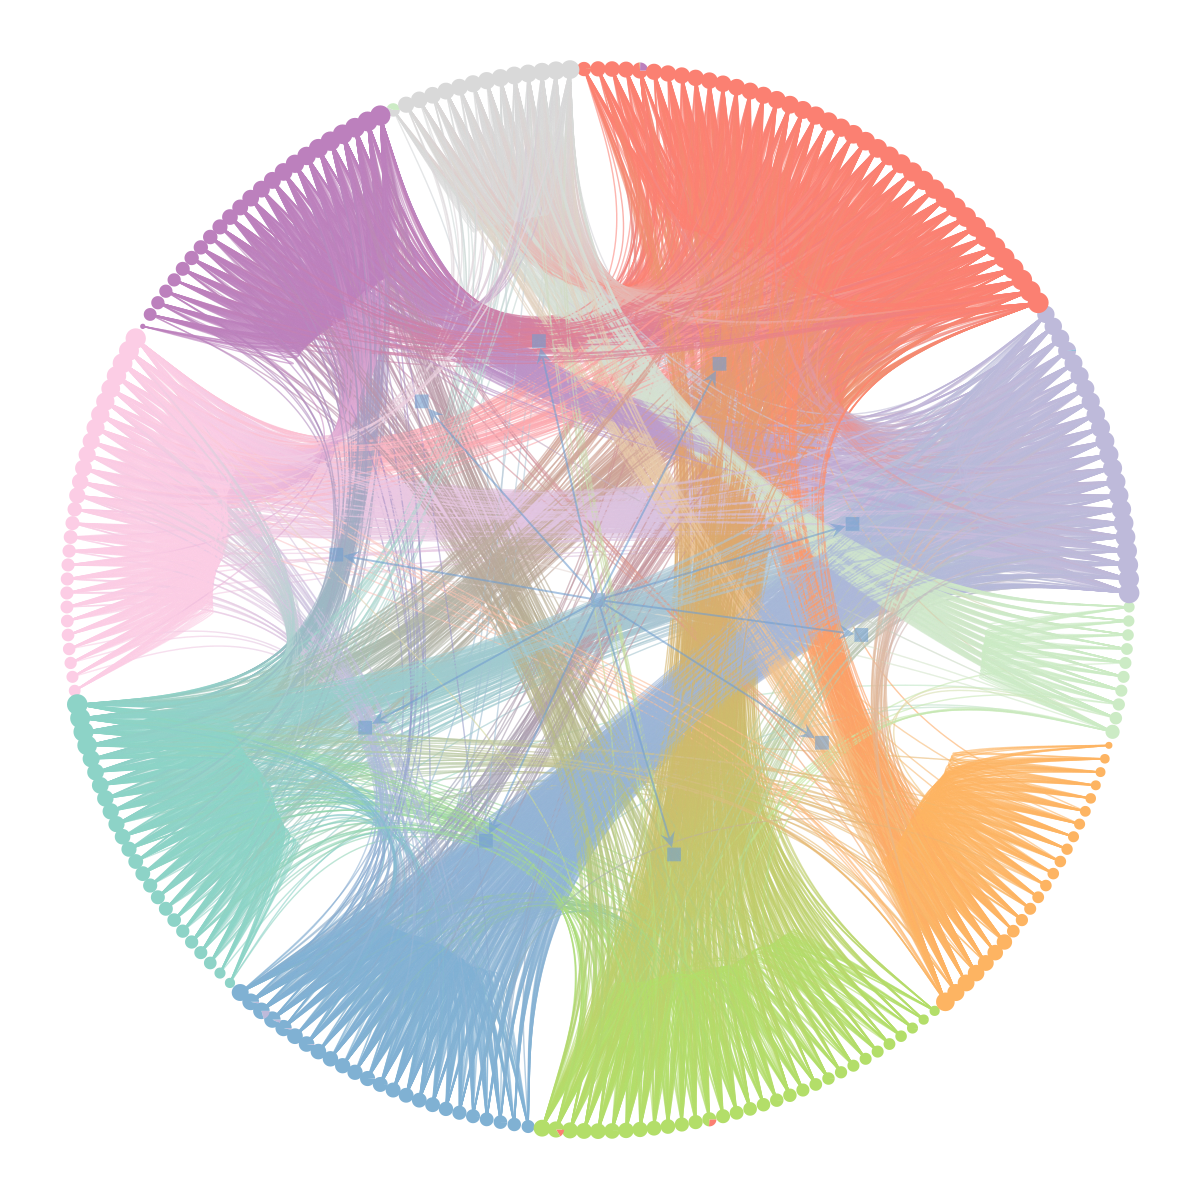
\includegraphics[width=0.28\linewidth]{img/school-graph.png}
	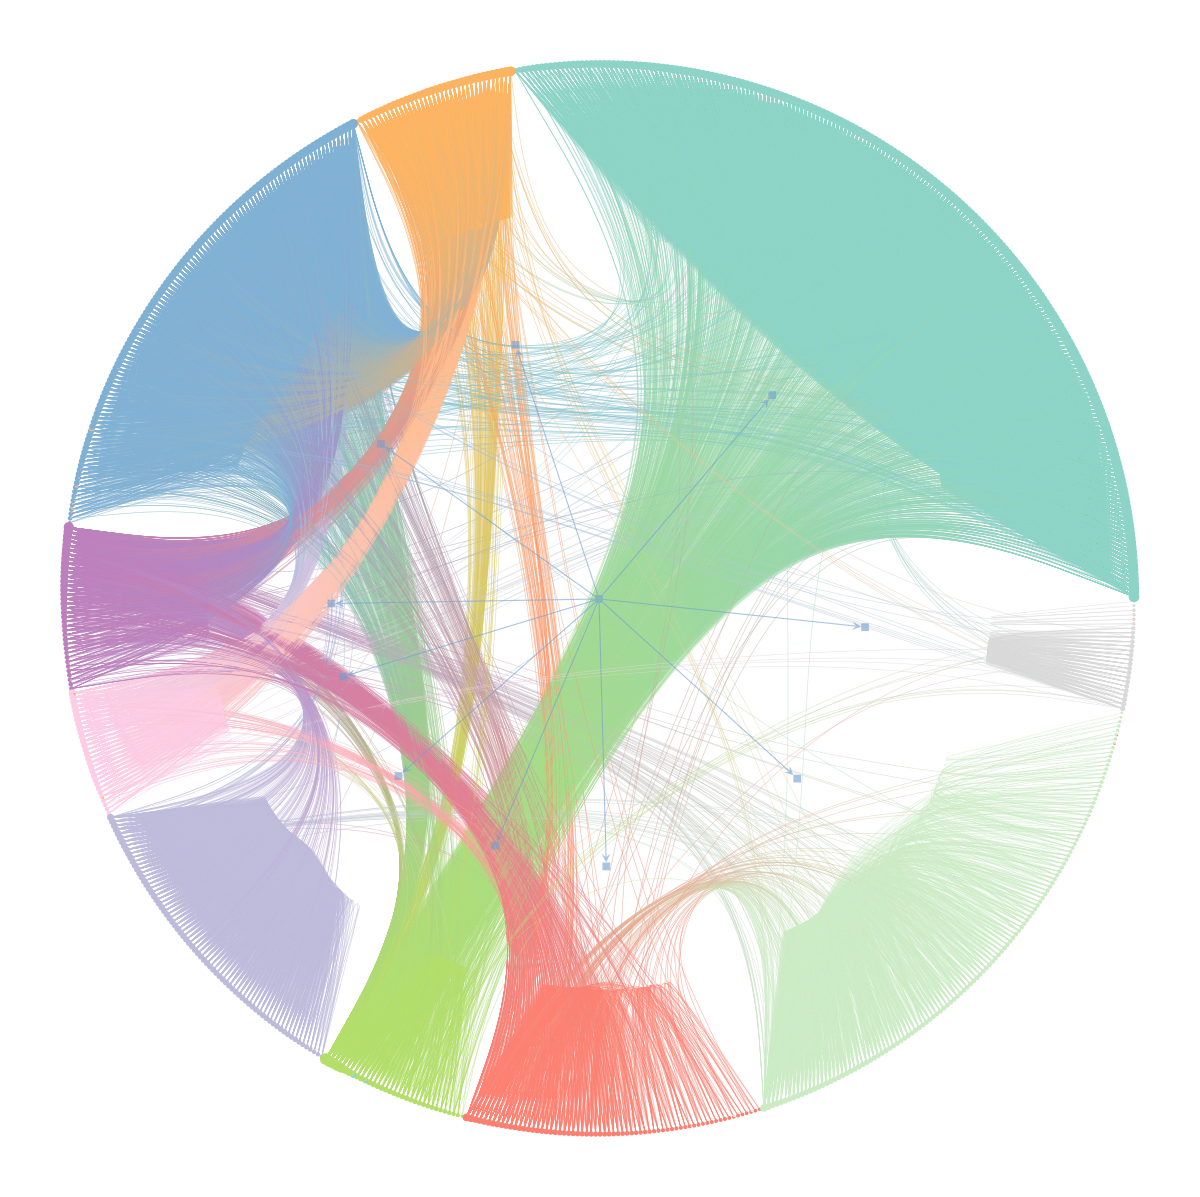
\includegraphics[width=0.28\linewidth]{img/fb-graph.png}
	\caption{Networks laid out and coloured according to inferred block memberships. Left to right: Polbooks, Krebs (2004); Primary School, Stehle et al (2011); Facebook Egonet, Leskovec and Mcauley (2012).}
	\label{fig:graphs-all}
\end{figure}

\clearpage